Considere un circuito RLC como el mostrado en la Figura 23, cuyo comportamiento, considerando como entrada el voltaje $V_g(t)$ de la fuente y como salida el voltaje en el capacitor $V_c(t)$, está dado por la ecuación diferencial de segundo orden

\begin{equation}
	\frac{d^2V_c(t)}{dt^{2}} +\frac{L}{R}+\frac{1}{LC} V_g(t)=\frac{1}{LC} V_g(t)
\end{equation}

\noindent considere que $\frac{R}{L}=1$ y $\frac{1}{LC}=5$

\begin{itemize}
\item Resuelva la ecuación diferencial utilizando los métodos analíticos disponibles en el software especializado que esté utilizando, escriba la solución y grafíquela, muestre los resultados en el siguiente cuadro
\end{itemize}

\noindent \textbf{Solución analítica del circuito:}

Empezamos por la sustitución de los valores dados en el ejercicio, donde $\frac{R}{L}=1$ y $\frac{1}{LC}=5$. Con esto podemos reescribir nuestra ecuación de la siguiente forma:

\begin{equation}
	\frac{d^2V_c(t)}{dt^2}+\frac{dV_c(t)}{dt}+5V_g(t)=5V_g(t)
\end{equation}

\noindent Realizamos la sustitución de $V_c(t)=y(t)$ y $V_g(t)=x(t)$

\begin{equation}
	\frac{d^2y(t)}{dt^2}+\frac{dy(t)}{dt}+5y(t)=5x(t)
\end{equation}

\noindent Con dichos cambios ya podemos empezar a aplicar la transformada de Laplace a ambos lados de la ecuación

\begin{equation}
	\Laplace\{{\frac{d^2y(t)}{dt^2}+\frac{dy(t)}{dt}+5y(t)}\}=\Laplace\{{5x(t)}\}
\end{equation}

\begin{equation}
	s^2Y(s)+sY(s)+5Y(s)=5X(s)
\end{equation}

\noindent Factorizamos $Y(s)$ y $X(s)$

\begin{equation}
	Y(s)(s^2+s+5)=5X(s)
\end{equation}

\noindent Si reacomodamos la expresión finalmente llegamos a la función de transferencia

\begin{equation}
	H(s)=\frac{Y(s)}{X(s)}=\frac{5}{(s^2+s+5)}
\end{equation}

\noindent Si consideramos la entrada un escalor, es decir que $X(s)=1$ simplificamos la expresión a 

\begin{equation}
	Y(s)=\frac{5}{(s^2+s+5)}
\end{equation}

\noindent Una vez teniendo la transformada de Laplace podemos aplicar la antitransformada para llegar a la ecuación solución del sistema.

\begin{equation}
	\Laplace^-1\{Y(s)\}=\Laplace^-1\{\frac{5}{(s^2+s+5)}\}
\end{equation}

\begin{equation}
	y(t)=\frac{10\sqrt(19)e^\frac{-t}{2}sin(\frac{\sqrt(19)t)}{2})}{19}
\end{equation}

\noindent\textbf{Representación grafica: }

\noindent 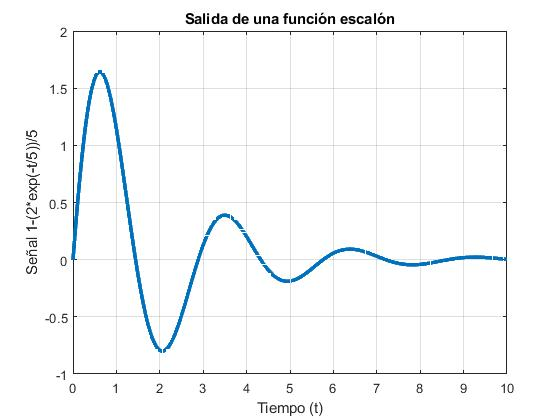
\includegraphics[scale=0.6]{./img2/salidaejercicio1}

\begin{itemize}
	\item Considerando un periodo de muestreo de $ T_s = 1 $ y utilizando el método de discretización mediante
	diferencias finitas, encuentre la ecuación en diferencias asociada y resu´elvala utilizando el método de recurrencia. Compare los resultados gr´aficos de la versi´on de tiempo continuo y la de tiempo discreto para diferentes valores del periodo de muestreo (disminúyalo en un punto decimal hasta $T_s = 0,0001$).
\end{itemize}

Empezaremos por encontrar la ecuación en diferencias.Para esto tendremos que utilizar la definición que nos permite transformar de una ecuación diferencial a una en diferencias:

\begin{equation}
\frac{dy}{dx}=\frac{y(t)-y(t-T_s)}{T_s}
\end{equation}

\noindent e igualmente usaremos la que nos permite pasar de una diferencial de segundo grado a su equivalente en diferencias:

\begin{equation}
\frac{d^2y}{dt^2)}=\frac{y(t)-2y(t-T_s)+y(t-2T_s}{T_s^2}
\end{equation}

\noindent Tras sustituir ambas definiciones llegamos a:

\begin{equation}
\frac{V_c(t)-2V_c(t-T_s)+V_c(t-2T_s)}{T_s^2}+\frac{R}{L}\frac{V_c(t)-V_c(t-T_s)}{T_s}+\frac{1}{LC}V_c(t)=\frac{1}{LC}V_g(t)
\end{equation}

\noindent Aplicamos las equivalencias que nos dieron al inicio de la práctica $\frac{R}{L}=5$, $\frac{1}{LC}=5$, $V_c(t)=y(t)$ y $V_g(t)=x(t)$

\begin{equation}
\frac{y(t)-2y(t-T_s)+y(t-2T_s)}{T_s^2}+\frac{y(t)-y(t-T_s)}{T_s}+5y(t)=5x(t)
\end{equation}

\noindent \textbf{Salida con $T_s=1$}

\noindent 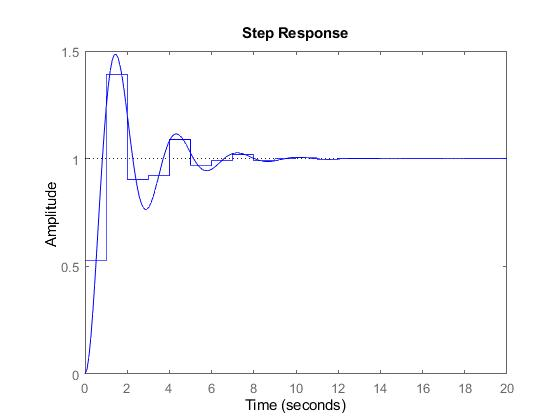
\includegraphics[scale=0.6]{./img2/SalidaTs1}

\noindent \textbf{Salida con $T_s=0,0001$}

\noindent 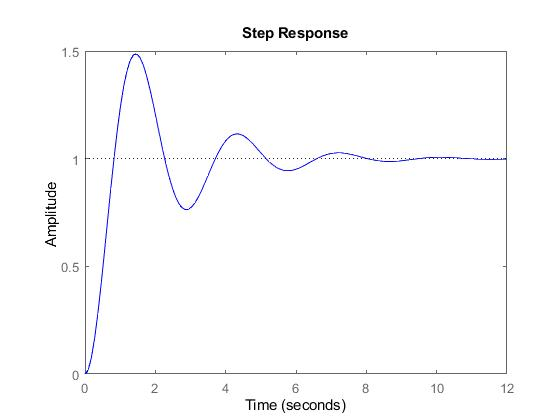
\includegraphics[scale=0.6]{./img2/SalidaTs00001}

Para la obtención de las gráficas anteriores se usaron los siguientes comandos de Matlab:

\begin{itemize}
\item Ts=1
\item Hs=tf([5],[1 1 5])
\item Hz=c2d(Hs,Ts,'foh')
\item step(Hs,'-',Hz,'-')
\end{itemize}


Como podemos concluir de observar ambas gráficas, la importancia de $T_s$ radica en que mientras más se acerque su valor a cero mejor será la aproximación de la solución de ecuaciones por diferencias a la solución de la ecuación en tiempo contínuo. Esto mismo lo podemos ver al hacer $T_s=0.0001$ parece que las gráficas se sobreponen, mientras que en $T_s=1$ se ve claramente la diferencia entre ambas gráficas. Cabe aclarar que la gráfica obtenida mediante la solución de diferencias finitas nunca va a ser la misma que la de tiempo continuo sin importar cuanto se disminuya $T_s$

\begin{itemize}
	\item Obtenga la función de transferencia del sistema de tiempo continuo.
	\item Utilizando $ T_s = 1 $:
\end{itemize}

\begin{equation}
	H(s)=\frac{Y(s)}{X(s)}=\frac{5}{(s^2+s+5)}
\end{equation}


\textbf{A)} Obtenga la función de transferencia de tiempo discreto de la ecuación en diferencias que resultó en	el punto anterior.

A partir de la ecuación obtenida en el ejercicio anterior

\begin{equation}
\frac{y(t)-2y(t-T_s)+y(t-2T_s)}{T_s^2}+\frac{y(t)-y(t-T_s)}{T_s}+5y(t)=5x(t)
\end{equation}

Podemos llegar a que si $T_s=1$ nuestra ecuación por diferencias es la siguiente:



\begin{equation}
\frac{0.5252z^2+1.231z+0.3053}{z^2 +0.6936x + 0.3679}
\end{equation}

Dicha ecaución es obtenida en Matlab tras usar los siguientes comandos.

\begin{itemize}
\item Ts=1
\item Hs=tf([5],[1 1 5])
\item Hz=c2d(Hs,Ts,'foh')
\end{itemize}

\textbf{B)}  Obtenga la función de transferencia de tiempo discreto a partir de la función de transferencia de tiempo continuo del sistema utilizando un diferenciador discreto, ¿cómo son las funciones de transferencia obtenidas en este punto y el anterior? ¿qué puede concluir?

Como ya habíamos mencionado antes, la función de transferencia en tiempo discreto utilizando un diferenciador discreto es la siguiente:

\begin{equation}
\frac{0.5252z^2+1.231z+0.3053}{z^2 +0.6936x + 0.3679}
\end{equation}

La comparación entre la obtención de la función de transferencia con y sin diferenciador se ve en las gráficas de la siguiente pregunta. Lo que se puede observar es que mediante el uso del diferenciador, la ecuación y su gráfica se acercan más a la ecuación y gráfica de la respuesta en tiempo contínuo, es decir, la presencia del diferenciador hace más exacta la aproximación en tiempo discreto.

\begin{itemize}
	\item Grafique en una sola figura la respuesta al impulso del sistema de tiempo continuo, y las dos aproximaciones
	de tiempo discreto.
\end{itemize}

Para esto se generaron dos gráficas: una sin diferenciador discreto y una con diferenciador discreto, siendo representadas por las curvas roja y amarilla respectivamente. Cabe mencionar que las curvas son la respueta al impulso.

\noindent \textbf{Salida con $T_s=1$}

\noindent 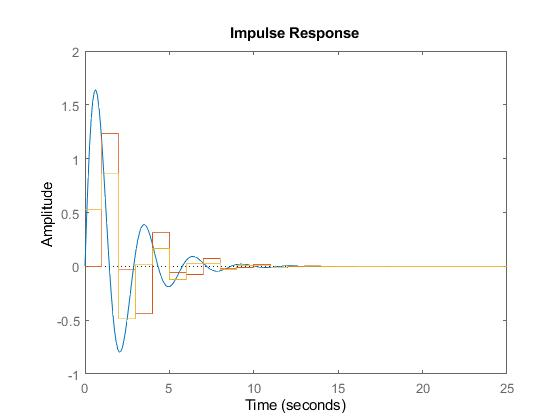
\includegraphics[scale=0.6]{./img2/SalidaTs1DosHz}

La obtención de la gráfica anterior se realizó con la siguiente serie de comandos

\begin{itemize}
\item Ts=1
\item Hs=tf([5],[1 1 5])
\item Hz=c2d(Hs,Ts)
\item Hz2=c2d(Hs,Ts,'foh')
\item impulse(Hs)
\item hold on
\item dimpulse(Hz,Ts)
\item hold on
\item dimpulse(Hz2,Ts)
\end{itemize}

\begin{itemize}
	\item Disminuya el tiempo de muestreo hasta obtener una aproximación adecuada de la respuesta del sistema
	y grafique la comparación. ¿Qu´e aproximación resultó mejor?
\end{itemize}

Para obtener una aproximación adecuada se disminuyó el valor de $T_s$ a 0.0001, generando la siguiente 
\newline

\noindent \textbf{Salida con $T_s=0.0001$}

\noindent 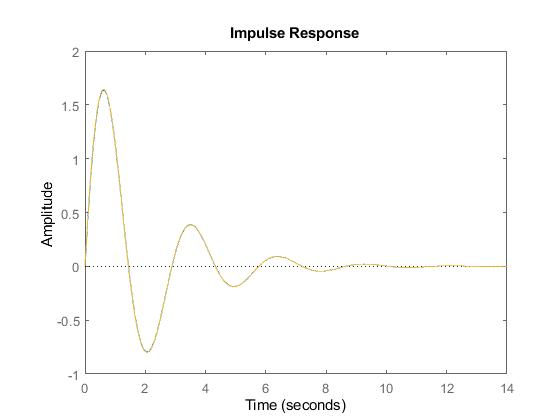
\includegraphics[scale=0.6]{./img2/SalidaTs00001DosHz}

Debido a la gran aproximación de ambas gráficas se requiere de un acercamiento para poder observar las diferencias entre la gráfica generada con diferenciador (amarilla) y la generada sin diferenciador (roja).

\noindent 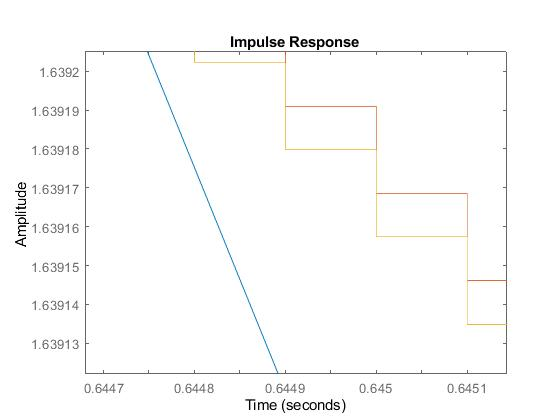
\includegraphics[scale=0.6]{./img2/SalidaTs00001DosHzAcercamiento}

Gracias a este acercamiento podemos apreciar que la gráfica que se acerca más a la de tiempo continuo (azul) es la que utiliza un diferenciador (amarilla). Para esto utilizamos los comandos:

\begin{itemize}
\item Ts=0.0001
\item Hs=tf([5],[1 1 5])
\item Hz=c2d(Hs,Ts)
\item Hz2=c2d(Hs,Ts,'foh')
\item impulse(Hs)
\item hold on
\item dimpulse(Hz,Ts)
\item hold on
\item dimpulse(Hz2,Ts)
\end{itemize}

\textbf{Comparacion de solución de tiempo continuo y solución de tiempo discreto utilizando funciones de tranferencia para diferentes valores de tiempo de muestreo }

{\Large Control discreto de un sistema de tiempo continuo.}

Considere un sistema lineal e invariante en el tiempo representado por la siguiente función de transferencia

\begin{equation*}
	G(s)=\frac{1}{s(s+3)}
\end{equation*}

\begin{itemize}
	\item Determine la estabilidad del sistema.
Para poder determinar la estabilidad del sistema, vamos a ver con MATLAB en donde se encuentran sus Polos. Para ello vamos a escribir los siguientes comandos.\\
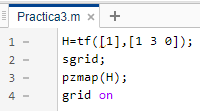
\includegraphics[scale=1]{cod1.png}\\
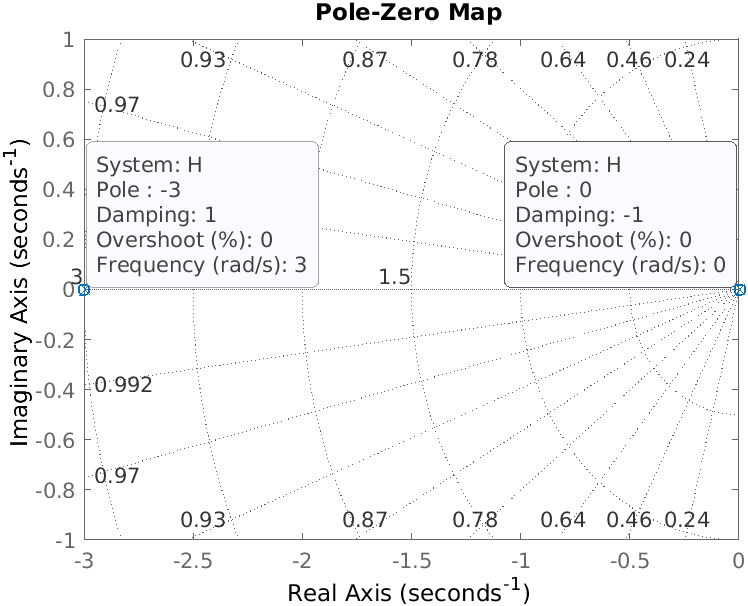
\includegraphics[scale=1]{G1.png} \\
Como se puede ver un polo esta en s=-3, pero el otro polo esta en s=0, por lo que no podemos decir si el sistema es estable o no. Ya que para que un sistema sea estable TODOS sus polos deben de estar en la parte izquierda del plano S. Por lo que primero veremos su respuesta al escalón para así poder determinar si el sistema es estable o no.

	\item Utilizando el software especializado de su preferencia, determine la respuesta al escalón del sistema y describa como es su comportamiento.
Para determinar la respuesta al escalón del sistema vamos a agregar el siguiente comando al código anterior: step(H,'-')\\
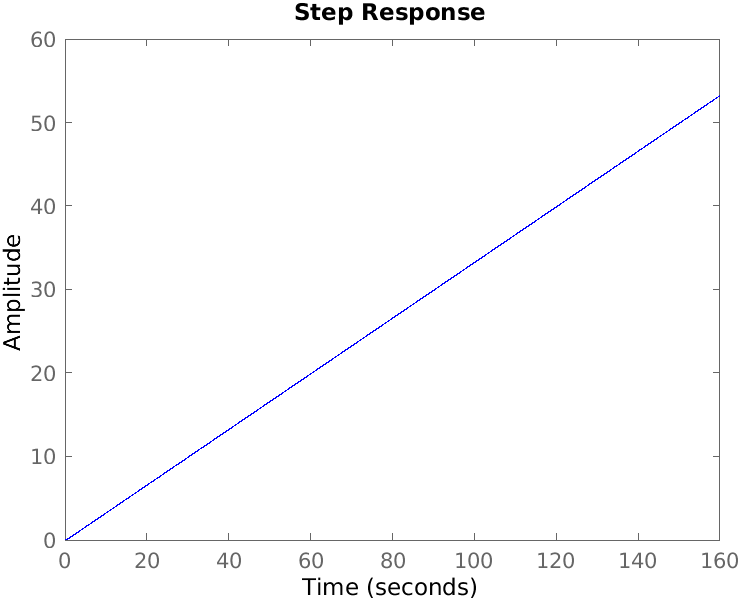
\includegraphics[scale=1]{G2.png} \\
Al analizar esta gráfica podemos ver que no tiene fin, en otras palabras la gráfica no tiene limite, ya que solamente es creciente conforme va avanzando en el eje X positivo. Por lo que podemos concluir a la pregunta anterior que NO es estable el sistema.

\end{itemize}

\begin{figure}[H]
	\centering
	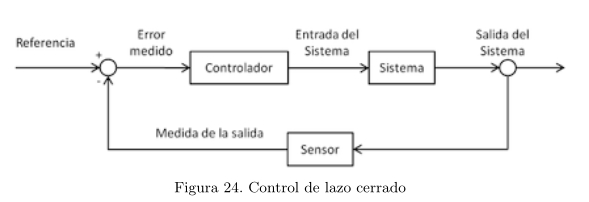
\includegraphics[scale=0.7]{img2/fig24}
	\label{fig:fig24}
\end{figure}

\textbf{Respuesta al escalón del sistema a controlar}

\begin{itemize}
	\item Cuando se desea cambiar el comportamiento de un sistema se debe implementar un controlador de lazo
	cerrado, el cual compara la se˜nal de salida del sistema con la se˜nal de referencia y con base en esta se˜nal
	de error calcula la entrada del sistema para que se obtenga el comportamiento deseado, de acuerdo con
	el diagrama de bloques mostrado en Figura 24. El modo m´as simple de control consiste en el control
	proporcional, el cual realimenta un término proporcional del error de salida, es decir,
\end{itemize}

\begin{equation*}
	u_c=K(r-y)
\end{equation*}

La conexión de la Figura 24 se denomina conexión en retroalimentación negativa, y es posible determinar la función de transferencia correspondiente mediante software especializado, para lo cual se deben definir
previamente las funciones de transferencia del controlador, del sistema y del sensor. Considerando la función de transferencia del sistema, la del controlador como C(s) = K y la del sensor H(s) = 1, determine
la función de transferencia de lazo cerrado Gc(s) correspondiente. ¿Cómo son los polos del sistema? ¿Qué puede decir de la estabilidad del mismo?
$$E(s)=R(s)-Y(s)$$
Donde: E(s) es el error medido, R(s) es la referencia y Y(s) es la salida.
$$H(s)=frac{Y(s)}{X(s)}$$
$$Y(s)=H(s)KX(s)$$
Si E(s)=X(s):
$$Y(s)=H(s)KE(s)$$
$$Y(s)=\frac{1}{s(s+3)}KE(s)$$
$$Y(s)=\frac{KE(s)}{s(s+3)}$$
$$E(s)=\frac{Y(s)(s(s+3))}{k}$$
Si $E(s)=R(s)-Y(s)$
$$R(s)-Y(s)=\frac{Y(s)(s(s+3))}{k}$$
$$KR(s)-KY(s)=Y(s)(s(s+3))$$
$$KR(s)=Y(s)(s(s+3)+K)$$
$$G_{c}(s)=\frac{Y(s)}{R(s)}=\frac{K}{s(s+3)+K}$$
Función de transferencia de lazo cerrado:
$$G_{c}(s)=\frac{Y(s)}{R(s)}=\frac{K}{(s(s+3)+K)}$$	
Si k=1:
$$G(s)=\frac{1}{(s(s+3)+1)}$$	
$$G(s)=\frac{1}{s^{2}+3s+1}$$	
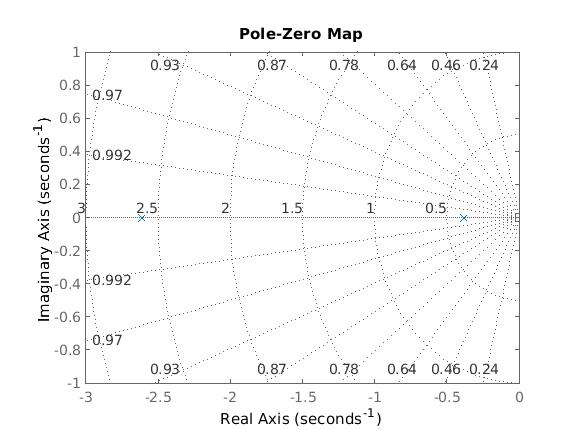
\includegraphics[scale=0.5]{./img2/G3.jpg}\\ 
Polos: $P_{1}=-2.618$ y $P_{2}=-0.382$. Por lo tanto es estable el sistema.\\
Respuesta al escalón del sistema:\\
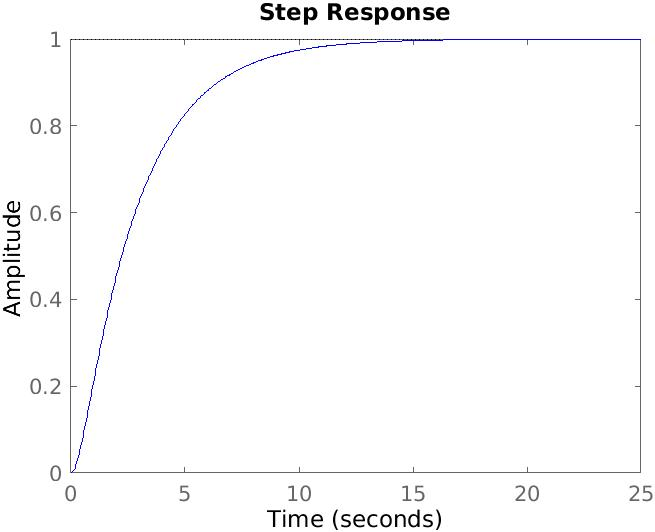
\includegraphics[scale=0.4]{./img2/G5.jpg}\\
Si k=-10:
$$G(s)=\frac{-10}{(s(s+3)-10)}$$	
$$G(s)=\frac{-10}{s^{2}+3s-10}$$
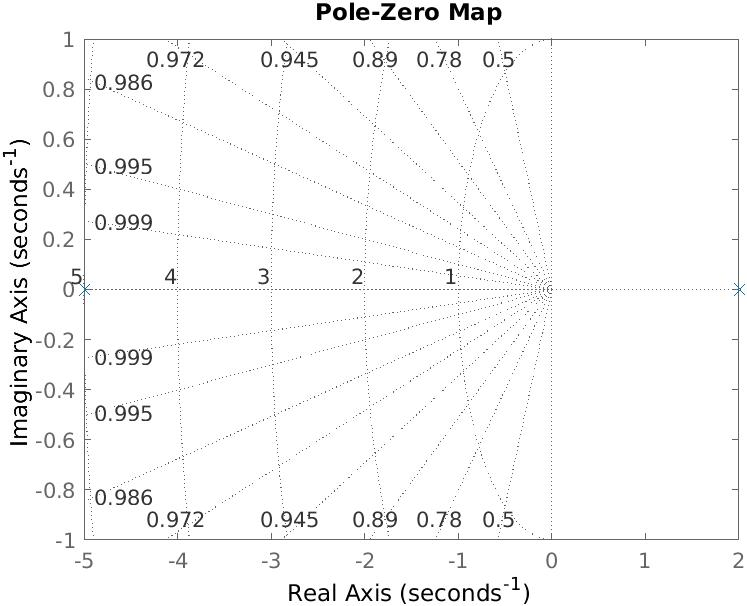
\includegraphics[scale=0.36]{./img2/G4.jpg}\\ 	
Polos: $P_{1}=-5$ y $P_{2}=2$. Por lo tanto es inestable el sistema.\\
Respuesta al escalón del sistema:\\
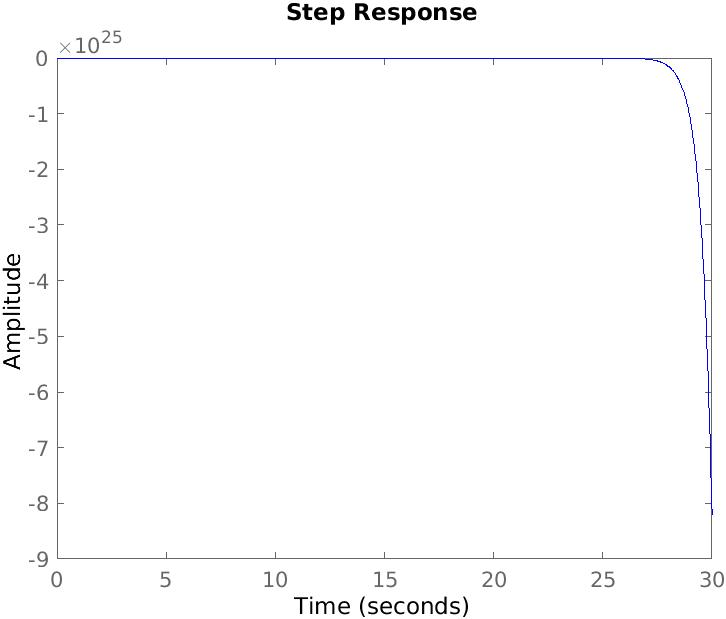
\includegraphics[scale=0.36]{./img2/G6.jpg}\\
¿Cómo son los polos del sistema? Dependiendo del valor de K los polos del sistema van a variar. Por lo que pueden volver estable o inestable al sistema.\\
¿Qué puede decir de la estabilidad del mismo? Lo que podemos ver con estos dos valores de K, es que dependiendo de su valor, se modificará la entrada del sistema, volviéndose estable o inestable el sistema.

\begin{itemize}
	\item A partir de las funciones de transferencia de lazo abierto y de lazo cerrado en tiempo continuo obtenga las versiones de tiempo discreto. Realice lo anterior utilizando los procedimientos presentados en la
	Introducción Teórica y el software especializado de su elección. Reporte sus resultados a continuación.
\end{itemize}

\textbf{Respuesta al escalón del sistema con control}

\begin{itemize}
	\item Determine los polos de lazo abierto y de lazo cerrado de tiempo discreto y caracterice la estabilidad de
	cada uno de estos. Determine la respuesta al escalón de ambos sistemas utilizando software especializado.
	Escriba sus resultados a continuación y las gráficas obtenidas en los espacios correspondientes.
\end{itemize}
\begin{figure}[H]
	\centering
	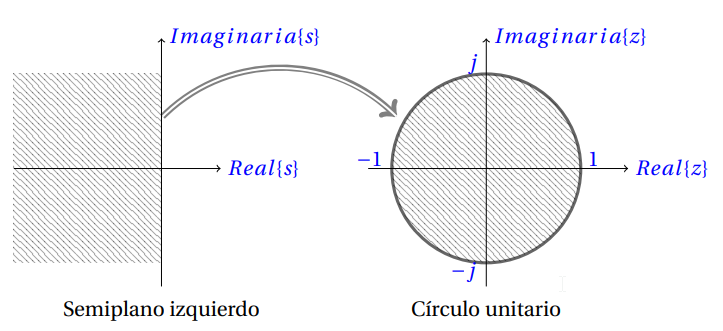
\includegraphics[width=0.7\linewidth]{img2/000004}
	\caption{Descripción}
	\label{fig:000004}
\end{figure}

\textbf{Respuesta al escalón del sistema en tiempo discreto}

\textbf{Respuesta al escalón del sistema de control en tiempo discreto}